\subsection{bomb\_tansaction.sh}
bomb\_tansaction.sh is a custom shell script that was used to test for vulnerabilities regarding SQL transactions and function execution limits.\\
It works by execution a number of transactions supplied by a text file with tans using curl all at once (in the background).
One can then check if the sent and revieved money are equal and if there is any action by the app if all codes where used.
\begin{figure}[ht]
	\centering
	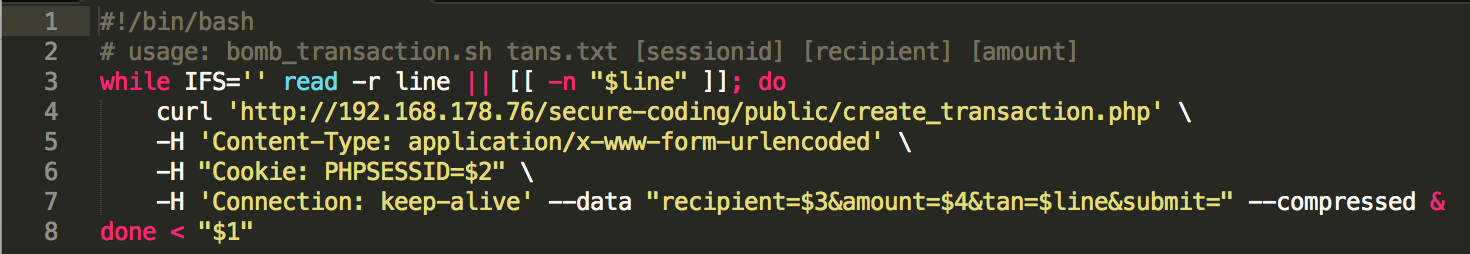
\includegraphics[width=.8\linewidth]{figures/tool_bomb_transaction.png}
	\caption{The tool simply loops through a text file with tans and performs parallel curl requests}
	\label{fig:tool_bomb_transaction}
\end{figure}